\documentclass[11pt]{article}
\usepackage[margin=1in]{geometry}
\usepackage{amsmath}
\usepackage{graphicx}
\usepackage{booktabs}
\usepackage{xcolor}
\usepackage[hidelinks]{hyperref}
\usepackage{caption}
\captionsetup{font=small}
\emergencystretch=3em

\newcommand{\code}[1]{\texttt{#1}}

\title{Accelerometer sample timing: dropped samples and biased frequencies}
\author{Ilan Upfal}
\date{28 October 2026}

\begin{document}
\maketitle

\section*{Summary}

The accelerometer board samples at the configured 1600\,Hz, but our capture
loop only saves about 1250 samples per second. Each read pulls at most 84
samples off the board and takes about 67\,ms, while the sensor produces
about 107 samples in that time. So about 23 samples (22\%) are lost between
every pair of batches. The overrun counter that would record this is never
logged.

Every spectral script treats the saved samples as one evenly spaced stream,
so the frequencies are wrong. With the assumption used in
\code{extract\_run\_summary.py} (even spacing at the measured $\approx$1250\,Hz
rate), the first flap mode of the DTU10MW rigid-4k blade comes out at
\textbf{47.5\,Hz}. A high-speed video of the same ringdown, filmed at
4000\,fps, gives \textbf{62.7\,Hz}. If we place the samples at 1600\,Hz
within each batch and leave the gaps empty, the accelerometer gives
\textbf{62.5\,Hz}.

\begin{itemize}
  \item \textbf{Affected:} every frequency from \code{extract\_run\_summary.py}
        (\code{spectra.npz} and the \code{peak\_hz\_*} columns), every
        \code{plot\_psd.py} figure, and the ringdown spectra.
  \item \textbf{Not affected:} variances and the results built on them.
  \item \textbf{Fix for existing data:} rebuild the timing as described in
        Section~\ref{sec:fix}.
  \item \textbf{Fix for future runs:} make the read keep up with the sensor,
        and log the overrun counter (Section~\ref{sec:recs}).
\end{itemize}

\section{How the data are captured}

The capture loop (\code{collect\_accel\_for\_duration} in \code{main.py}; the
ringdown script calls the same code) repeatedly
\begin{enumerate}
  \item reads \code{REG\_AVAIL}, the number of sample sets waiting on the board;
  \item reads $\min(\text{avail}, \code{BULK\_MAX\_SETS})$ sets in one bulk
        Modbus transfer, where \code{BULK\_MAX\_SETS = 84} is fixed by the
        firmware;
  \item writes every row of that batch to the CSV with the same timestamp:
        the \code{perf\_counter()} reading taken just after the transfer.
\end{enumerate}
The CSV therefore has no per-sample time. A sample's true time can only be
inferred from which batch it is in and where it sits in that batch. The
loop never reads \code{REG\_OVERRUN} or the sample counter, although
\code{test\_modbus.py}'s stream mode does.

\section{Evidence that samples are dropped}

All numbers below come from the 61 files of
\code{data/DTU10MW\_rigid4k\_ringdown} (1 rest, 30 flap, 30 edge, 10\,s each,
ODR 1600\,Hz) and are reproduced by \code{make\_figures.py} in this folder.

\paragraph{Every batch is full.} Apart from the final batch of each file,
every batch contains exactly 84 samples, which is the maximum the firmware
allows. If the reader kept up, some reads would find fewer than 84
samples waiting. A permanently full read means the backlog never clears.

\paragraph{The read cycle is longer than the time to fill a batch.} The
mean time between reads is 67.3\,ms (median 67.0, standard deviation 2.8). At
1600\,Hz the sensor fills 84 slots in $84/1600 = 52.5$\,ms
(Figure~\ref{fig:batches}, left). Each cycle the sensor therefore produces
$0.0673 \times 1600 \approx 107.6$ samples and we keep 84, losing
$\approx$23.6.

\paragraph{The delivered rate matches.} Across all files the delivered rate
is 1249\,Hz (range 1229--1253\,Hz), i.e.\ 21.9\% below the ODR, and it falls
behind the 1600\,Hz line at a steady rate (Figure~\ref{fig:batches}, right).
The QC in \code{ring\_down\_aquire.py} already flags every trial with
``accel rate $<$ 90\% of ODR (dropped samples?)''.

\paragraph{Why the read is slow.} One batch is $84 \times 12$ registers
$\times$ 2 bytes $\approx$ 2\,kB, or $\approx$22\,ms on the wire at
921\,600\,baud. That leaves roughly 45\,ms of each cycle for the rest of
the loop, which includes the \code{REG\_AVAIL} poll, Modbus turnaround,
writing CSV rows one at a time, and the \code{on\_poll} live-plot callback.
We have not profiled the loop, but transfer time alone does not explain
the 67\,ms cycle.

\begin{figure}[t]
  \centering
  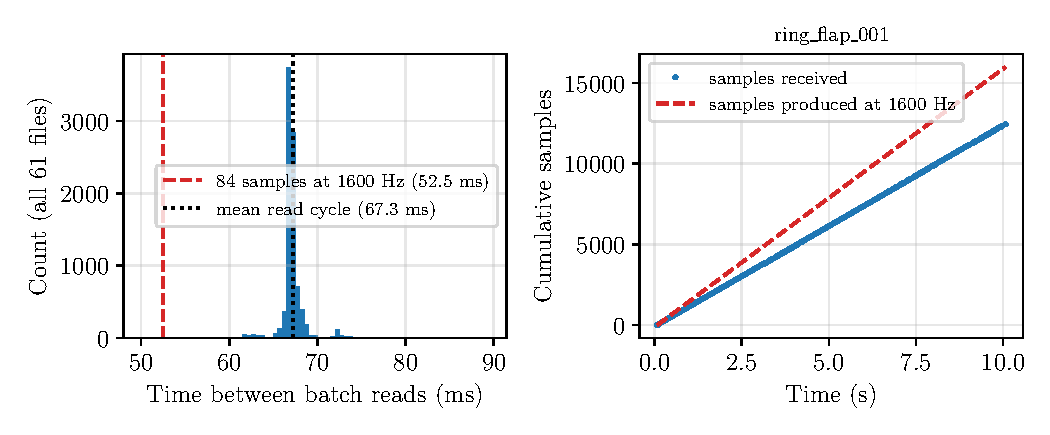
\includegraphics[width=\linewidth]{figs/batches.pdf}
  \caption{Left: time between batch reads over all 61 files; the dashed line
  is the time the sensor takes to produce one batch. Right: samples received
  versus samples produced at 1600\,Hz for one trial.}
  \label{fig:batches}
\end{figure}

\section{Independent reference: high-speed video}

A flapwise ringdown of the same blade was filmed with the Phantom camera at
4000\,fps (\code{DTU10MW\_rigid4k\_flapwise\_4.cine}). The tip deflection was
tracked with \code{beam\_tracker} (Figure~\ref{fig:video}). The camera's frame
timing comes from the file header and does not depend on our acquisition
code. The tip rings at \textbf{62.7\,Hz}, from both the spectrum and the zero
crossings of the first ten cycles. The next-largest peak, at 164.5\,Hz, is
about 1\% of the first mode's amplitude.

This comparison assumes the video and the accelerometer ringdowns use the
same blade and mounting.

\begin{figure}[t]
  \centering
  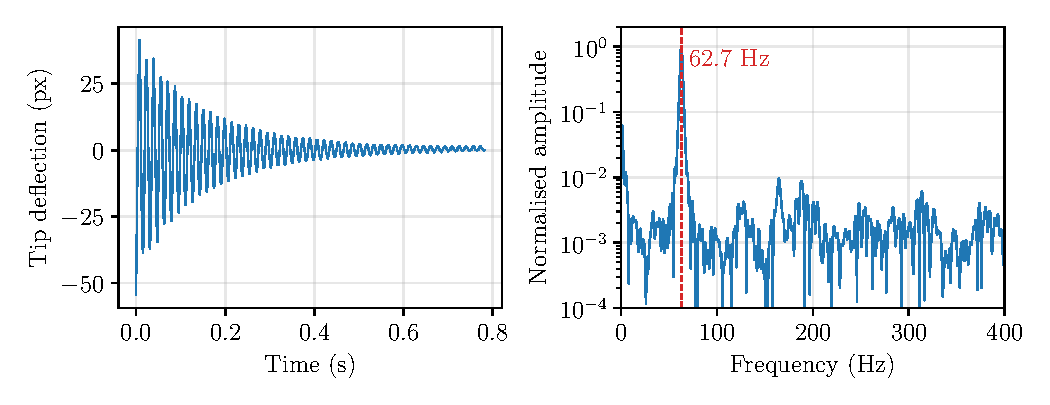
\includegraphics[width=\linewidth]{figs/video.pdf}
  \caption{High-speed video reference. Left: tracked tip deflection.
  Right: its amplitude spectrum (Hann window), normalised to the first mode.}
  \label{fig:video}
\end{figure}

\section{Why each timing assumption gives the frequency it does}
\label{sec:why}

The data are 84-sample runs taken at 1600\,Hz, one run every
$T_b = 67.3$\,ms, with gaps in between. Two things in a spectrum depend on
the timing:

\begin{itemize}
  \item \textbf{Within a batch,} consecutive samples are $1/1600$\,s apart.
        This sets roughly where the peak is (a broad envelope).
  \item \textbf{Between batches,} the phase is only sampled once per batch, at
        $f_b = 1/T_b = 14.9$\,Hz. A tone at $f$ is therefore indistinguishable
        from $f \pm n f_b$, which produces a comb of lines spaced $f_b$ apart.
        The highest line is the one nearest the centre of the envelope.
\end{itemize}

We compared three timing assumptions on the flap trials (median PSD of
\code{s4\_z}, the sensor nearest the tip; Figure~\ref{fig:methods}):

\begin{enumerate}
  \item \textbf{Even spacing at the delivered rate ($\approx$1250\,Hz).}
        Used in \code{extract\_run\_summary.py} ($f_s = n / t_\text{end}$)
        and \code{ring\_down\_aquire.py}, and implicitly by
        \code{\_reconstruct\_batch\_times} in \code{run\_loader.py}, which
        spreads each
        batch evenly back to the previous timestamp. The batch start times
        come out roughly right, so the comb sits at
        $62.7 \pm n \times 14.9$\,Hz. But samples within a batch are assumed
        $1/1250$\,s apart instead of $1/1600$, so the envelope is centred
        near $62.7 \times 1250/1600 \approx 49$\,Hz. The nearest comb line
        is $62.7 - 14.9 = 47.9$\,Hz. \textbf{Measured: 47.5\,Hz.}
  \item \textbf{Even spacing at 1600\,Hz, batches joined end to end.} Used
        in \code{explore.py} (section~9). The within-batch spacing is
        correct, so the envelope is centred at 62.7\,Hz. But the gaps are
        removed, so each 67.3\,ms batch cycle is squeezed into 52.5\,ms. The
        comb moves to $62.7 \times 67.3/52.5 = 80.4$\,Hz with spacing
        $1600/84 = 19.0$\,Hz, and its line nearest 62.7 is
        $80.4 - 19.0 = 61.4$\,Hz. \textbf{Measured: 60.8\,Hz}, about 3\% low.
  \item \textbf{1600\,Hz within each batch, gaps left empty.} Each sample is
        placed on the $1/1600$\,s grid: contiguous within its batch, with the
        last sample at the batch's read timestamp. The dropped samples stay
        as gaps and are masked out of the Welch estimate. Both the envelope
        and the comb are now centred on the true frequency.
        \textbf{Measured: 62.5\,Hz}, against the video's 62.7\,Hz and a
        0.78\,Hz frequency resolution.
\end{enumerate}

The predicted values (47.9 and 61.4\,Hz) match what was measured (47.5 and
60.8\,Hz), which supports this account of the timing. Method~3 still shows
the comb: weaker copies of the mode at $62.7 \pm 14.9$ and
$62.7 + 2 \times 14.9$\,Hz (dotted lines in Figure~\ref{fig:methods}). The
gaps are periodic, so these copies cannot be removed from the existing
data.

\begin{figure}[p]
  \centering
  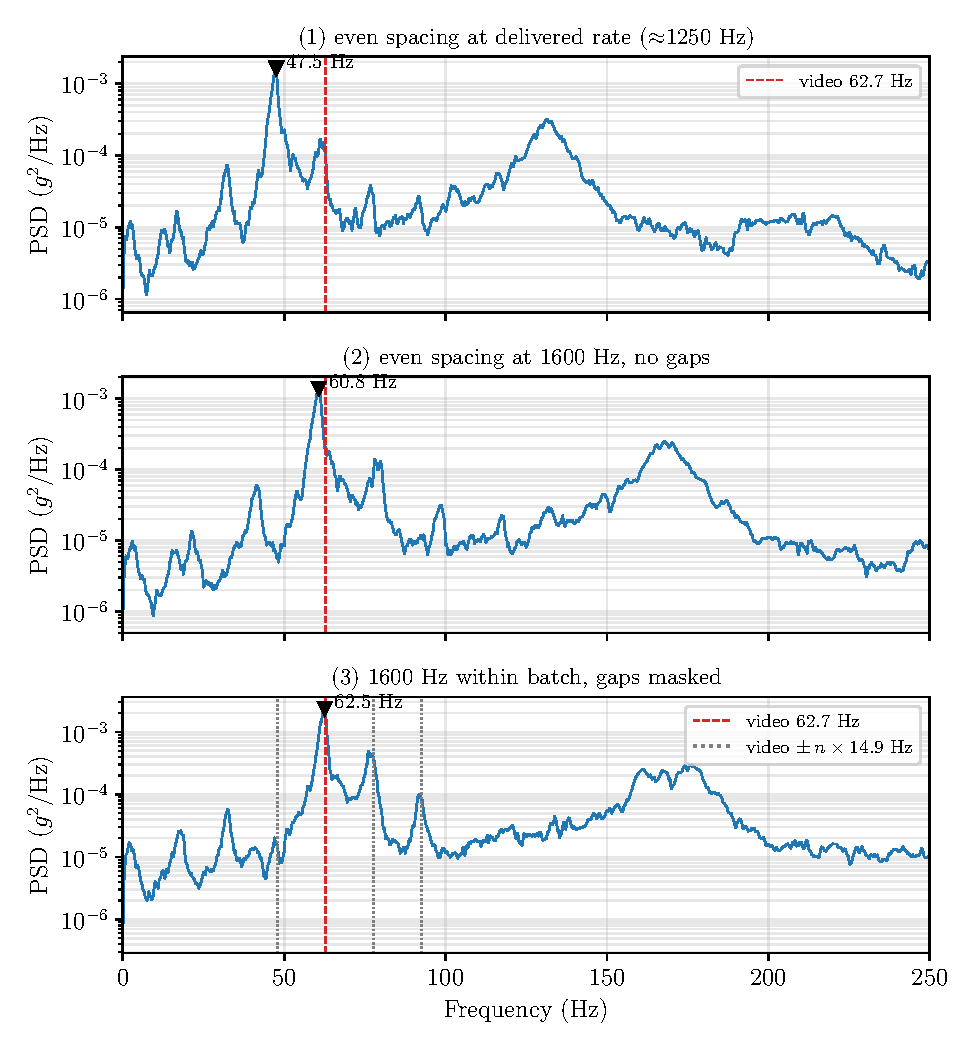
\includegraphics[width=0.92\linewidth]{figs/methods.pdf}
  \caption{Median PSD of \code{s4\_z} over the 30 flap trials under the three
  timing assumptions. Dashed red: video frequency. Dotted grey (bottom):
  the video frequency $\pm\,n \times 14.9$\,Hz, where the batch-gap copies
  of the mode are expected.}
  \label{fig:methods}
\end{figure}

\section{Corrected ringdown results}
\label{sec:fix}

\code{scripts/data\_analysis/ringdown/plot\_ringdown\_psd.py} now uses method~3.
Table~\ref{tab:peaks} compares the main peaks of the median PSDs before and
after. They do not all move by the same factor: each old peak landed on
whichever comb line was nearest its shifted envelope.

\begin{table}[h]
  \centering
  \begin{tabular}{llccc}
    \toprule
    Excitation & Where seen & Old (Hz) & Corrected (Hz) & Video (Hz) \\
    \midrule
    Flap & y, z, all sensors & 47--47.5 & 61.7--62.5 & 62.7 \\
    Flap & z               & 131--133 & 176--178 & (164.5, weak) \\
    Flap & y, z            & 218--226 & 275--285 & -- \\
    Flap & z, s1/s4        & 338      & $\approx$430 & -- \\
    Edge & y               & 98--100  & 118--121 & -- \\
    Edge & y               & 251--264 & 313--326 & -- \\
    Edge & y, s1/s4        & 453      & 577--597 & -- \\
    \bottomrule
  \end{tabular}
  \caption{Main peaks of the median PSDs (30 trials each), old timing
  (method~1) versus corrected timing (method~3).}
  \label{tab:peaks}
\end{table}

Peaks near 77 and 92\,Hz in the corrected spectra are $62.5 + 14.9$ and
$62.5 + 2 \times 14.9$\,Hz. They are copies of the first flap mode, not
separate modes. Any peak exactly 14.9\,Hz (or a multiple) from a stronger
peak should be treated the same way.

\begin{figure}[h]
  \centering
  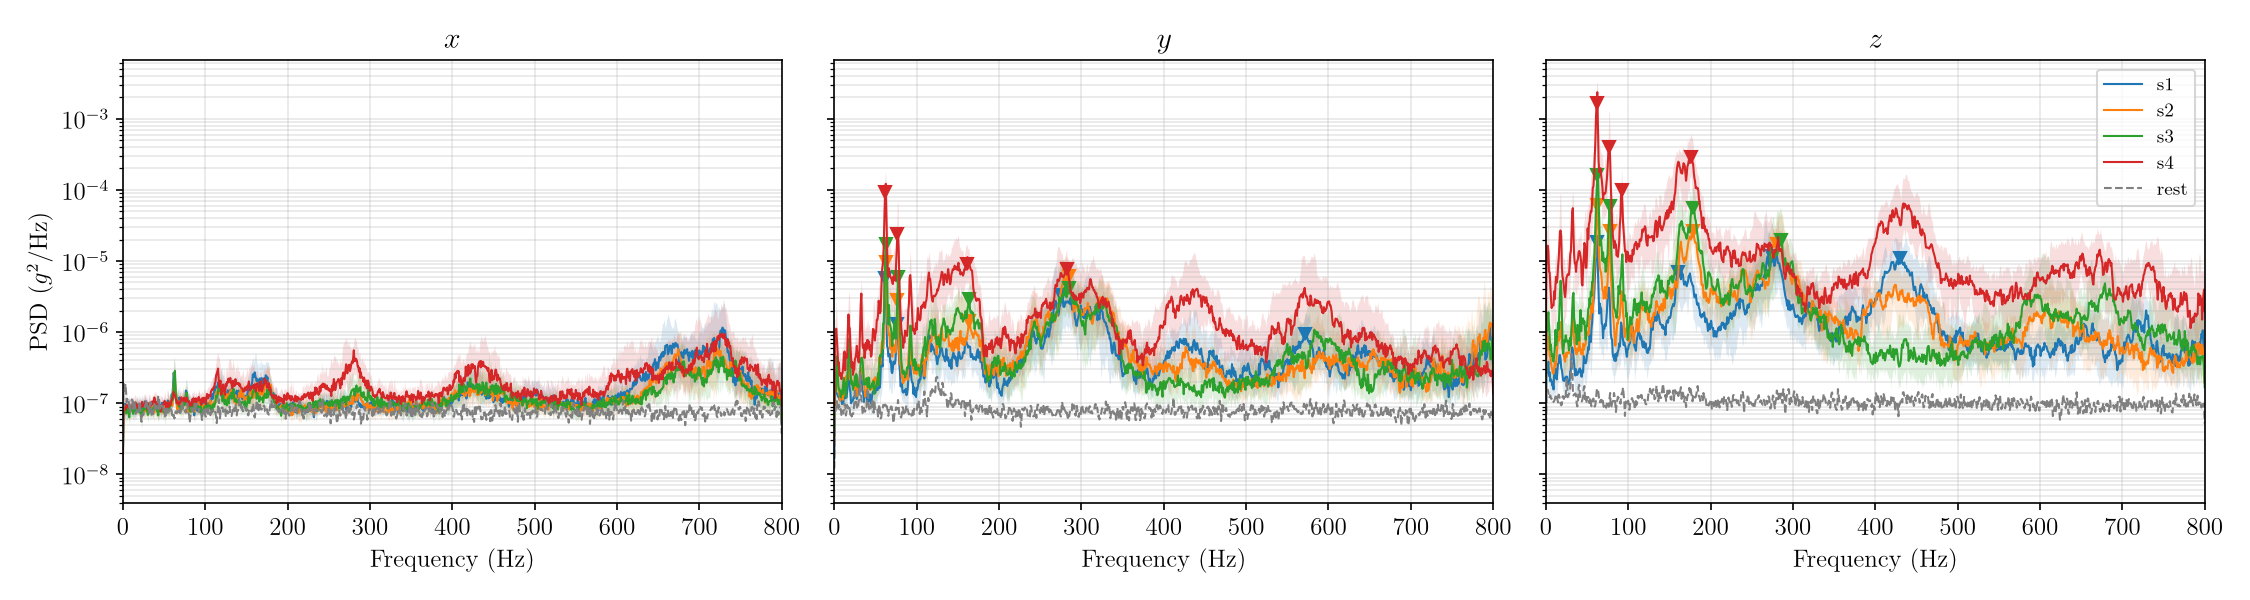
\includegraphics[width=\linewidth]{figs/psd_flap.png}\\[2pt]
  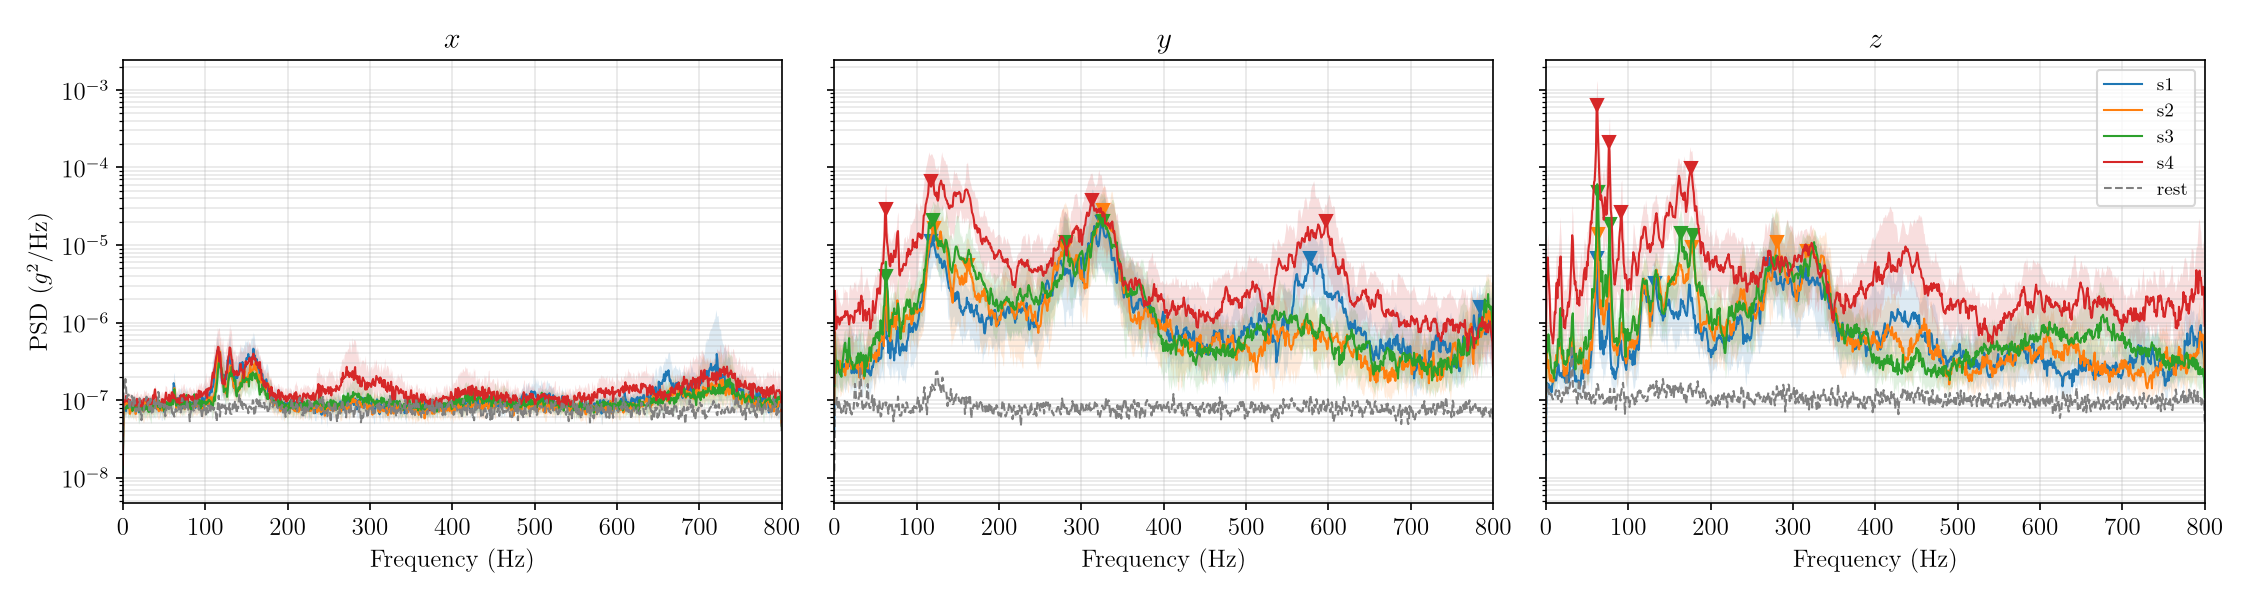
\includegraphics[width=\linewidth]{figs/psd_edge.png}
  \caption{Corrected median PSDs (method~3) for the flap (top) and edge
  (bottom) trials. Shading: 25--75th percentile across trials. Dashed grey:
  rest capture. Triangles: the four highest peaks per $y$/$z$ channel.}
  \label{fig:corrected}
\end{figure}

\paragraph{Limitations.}
\begin{itemize}
  \item Method~3 assumes the samples within a batch are consecutive sensor
        samples, with all losses between batches. We do not have the firmware
        source to confirm this; the agreement with the video is the support.
  \item Each batch is positioned by its read timestamp. That timestamp
        includes Python and serial latency, of order 1\,ms, so peaks at
        higher frequencies are smeared more.
  \item The 14.9\,Hz copies limit how weak a mode can be detected next to a
        strong one.
\end{itemize}

\section{What this affects in the shared scripts}

\begin{center}
\begin{tabular}{p{0.34\linewidth}p{0.24\linewidth}p{0.32\linewidth}}
  \toprule
  Script & Timing assumed & Effect \\
  \midrule
  \code{extract\_run\_summary.py} $\to$ \code{spectra.npz}, \code{peak\_hz\_*},
  \code{plot\_psd.py} & Method 1 & Frequencies 15--25\% low; the
  62.7\,Hz mode reads as 47.5\,Hz \\
  \code{utils/run\_loader.py} (time column) & Method 1 & Time axis stretched
  within batches; fine for plotting, wrong for spectra \\
  \code{explore.py} \S9 & Method 2 & About 3\% low; batch copies at 19\,Hz
  spacing \\
  \code{ring\_down\_aquire.py} QC & Method 1 & Rate only used for the
  warning and the RMS window \\
  Variance results & -- & Unaffected \\
  \bottomrule
\end{tabular}
\end{center}

The variance results are unaffected because a variance does not depend on
sample timing, and dropping a fixed 22\% of samples spread evenly through
the capture does not change it materially.

\section{Recommendations}
\label{sec:recs}

\begin{enumerate}
  \item \textbf{Log the overrun counter and sample counter on every read.}
        \code{REG\_OVERRUN} and \code{REG\_COUNTER\_L/H} are already exposed;
        \code{test\_modbus.py} reads them. Writing the counter into each
        batch would give the exact position of every sample and remove the
        guesswork in method~3.
  \item \textbf{Make the read keep up with the sensor.} The transfer itself
        needs only about 22 of the 67\,ms, so the cheapest fix is probably on
        the Python side: buffer rows and write the CSV after the capture,
        and call \code{on\_poll} less often or not at all during capture. If
        that is not enough, raise \code{BULK\_MAX\_SETS} in the firmware.
        Success means \code{REG\_AVAIL} sometimes reads below 84 and the
        delivered rate is $\approx$1600\,Hz.
  \item \textbf{Or lower the ODR.} At 800\,Hz the current loop keeps up
        ($\approx$54 samples per cycle), but the Nyquist frequency drops to
        400\,Hz. The flap peak near 430\,Hz and the edge peak near 580\,Hz
        would then fold back below 400\,Hz unless the sensor's
        anti-aliasing filter removes them.
  \item \textbf{Re-time the existing data.} Use method~3 in
        \code{extract\_run\_summary.py}, as in \code{plot\_ringdown\_psd.py},
        and regenerate \code{spectra.npz}.
\end{enumerate}

\end{document}
